\singlespacing

\mychapter{mygreen}{Méthodes}
  \sectiongreen*{Résumé}
    \begin{center}
      \begin{tabular}{c}
        \fcolorbox{mydarkgreen}{mylightgreen}{
        \begin{minipage}[][4cm][c]{0.8\linewidth}
          \sffamily
          Nous détaillerons ici notre méthode d'Intégration Transcriptome Interactome. J'ai choisi d'inclure dans cette section nos chapitres. Ces chapitres étant trop long, ils se trouvent dans les Annexes \ref{app:Garcia2011} \ref{app:Garcia2013}. L'algorithme ITI\index{ITI} sera décrit en détail, et les outils utilisés seront décrits briévement.
        \end{minipage}}\\
        \\[2ex]
        \begin{minipage}[][4cm][c]{0.9\linewidth}
          \mtcsetdepth{minitoc}{1}
          \minitoc
        \end{minipage}
      \end{tabular}
    \end{center}
    \newpage

\doublespacing

  \section{\textcolor{mygreen}{Les avantages de l'intégration de données}}

    \subsection{\textcolor{mygreen}{Les avantages de l'intégration de données d'expression des gènes et d'interactions protéine-protéine}}
      \mylettrine{R}{eprenant} les travaux de \citeauthor{vandevijver2002} et \citeauthor{Wang2005} sur l'analyse des jeux de données ayant permis l'établissement de signatures, \citeauthor{Chuang2007} rappellent les problèmes soulevés par ces prédentes études.
      Les ensembles de gènes permettant de prédire la rechute métastatique dans une étude sont moins efficaces quand il s'agit de prédire la rechute métastique sur le jeu de données de l'autre étude \citep{EinDor2006}.
      De plus, seulement trois gènes sont communs entre ces deux signatures à 70 et 76 gènes.
      L'hypothèse des gènes directeurs, étant probablement à l'origine du cancer, pertubant des gènes en aval est reprise ici pour expliquer ces différences entre ces deux ensembles de gènes.

      Pour circonvenir à ces inconvénients, l'utilisation de données d'interaction protéines-protéines permet de combiner les mesures d'expression des gènes issus de réseaux communs.
      Les biomarqueurs permettant d'établir une signature ne sont dans ce cas là plus les gènes ou les protéines, mais des sous-réseaux de protéines intergagissant ensebmble au sein du réseau des interactions proteines-protéines humain.

      Cette méthode a des avantages par rapport aux analyses classiques :
      \begin{itemize}
      \item Les sous-réseaux résultants procurent des modèles des méchanismes moléculaires sous-jascents de la métastase
      \item Les \emph{hubs} tels que \acs{TP53}, \acs{KRAS}, \acs{HRAS}, \acs{ERBB2}, non détectés par les analyses classiques, jouent un rôle central dans les réseaux en interconnectant un grand nombre de gènes.
      \item Les sous-réseaux identifiés sont signifiquativement plus reproductible entre différentes études que des boarqueurs individuels sélectionnés sans information sur l'interaction protéine-protéine.
      \item Une classification basée sur des réseaux permet d'obtenir une prédiction plus précise en sélectionnant les marqueurs sur un premier jeu de données d'entrainement et en les appliquant à un deuxième jeu de données de validation indépendant (cf figure~\ref{fig:Chuang2007figS1}).
      \end{itemize}

      \begin{figure}
        \centering
        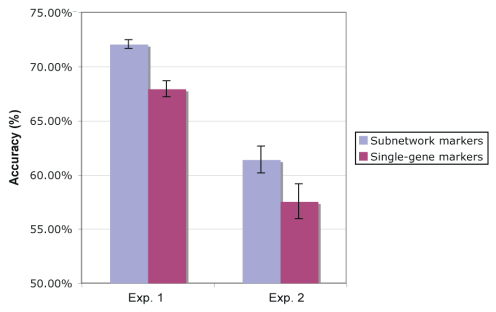
\includegraphics[width=\columnwidth]{figures/Chuang2007figS1.png}
        \caption{Avantages de l'intégration de données d'expression des gènes et d'interactions protéine-protéine sur la précision de la classification de la rechute métastatique par rapport à une analyse classique sur des données d'expression des gènes\citep{Chuang2007}.}
        \label{fig:Chuang2007figS1}
      \end{figure}

    \subsection{\textcolor{mygreen}{L'intégration de données d'expression des gènes et d'interactions protéine-protéine}}
      \mylettrine{C}{omme} nous l'avons vu précédemment, cette méthode a de grands avantages comparé aux méthodes classiques d'analyse de données d'expression des gènes.
      Les données d'interaction protéine-protéine sont utilisés pour assigner des ensembles de gènes sur des sous-réseaux.
      
      Les conditions cliniques des patients (ie métastatique ou non-métastatique) permettent de différencier les \acp{GEP} pour constituer une matrice d'activité du sous-réseau.

      Cette matrice d'activité sert à attribuer un score global à chaque sous-réseau, dérivé de l'expression de chacun des gènes le constituant.
      Des sous-réseaux générés par permutation permettent alors de sélectionner les sous-réseaux discrimants.
      Les sous-réseaux ainsi sélectionnés sont utilisés pour identifier les gènes causant la maladie, et la matrice d'activité du sous-réseau est utilisé pour entrainer un classifieur.

      \begin{figure}
        \centering
        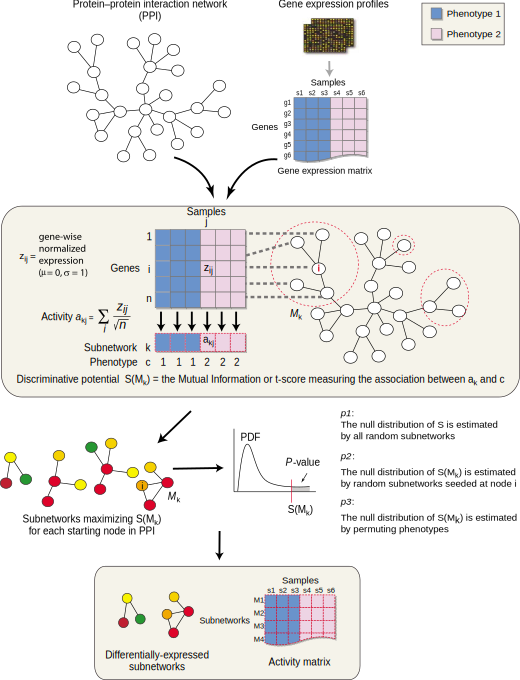
\includegraphics[width=\columnwidth]{figures/Chuang2007IntegrationAlgorithm.png}
        \caption{Algorithme détaillant l'intégration de données d'expression des gènes et d'interactions protéine-protéine\citep{Chuang2007}.}
        \label{fig:Chuang2007IntegrationAlgorithm}
      \end{figure}
    
%    \citep{Lazar2012}

  \section{\textcolor{mygreen}{L'\acl{ITIfr}}}

    \subsection{\textcolor{mygreen}{L'intégration massive de données d'expression des gènes et de données d'interactions protéine-protéine}}

      \mylettrine{L'}{intégration} massive de données d'expression des gènes et de données d'interactions protéine-protéine est la solution que nous avons dévelloppé pour circonvenir aux inconvénients des approches classiques des méthodes de prédiction de la rechute métastatique dans le cancer du sein.

      Nous avons vu précedemment que les approches classiques manquent de reproductibilités, dépendent grandement du jeu d'entrainement et sont moins performantes utilisées sur un jeu de données indépendant.

      Notre approche est une réimplémentation totale de l'algorithme développé par \citeauthor{Chuang2007}, avec la capacité supplémentaire de pouvoir prendre en compte plusieurs jeux de données d'expression des gènes.

      Nous allons d'abord détailler les données que nous avons utilisés tout au long de ces travaux.
      Et ensuite nous détaillerons l'algorithme.
  \section{\textcolor{mygreen}{Données d'expression des gènes}}\label{sec:GEP}

    \subsection{\textcolor{mygreen}{Constitution d'un compendium de données d'expression des gènes dans le cancer du sein}}
      \mylettrine{N}{ous} avons exploré les sites de dépôts de données publiques, ainsi que la littérature, et avons sélectionné les jeux de données dont les conditions cliniques étaient disponibles. Nous voulions séparer les patients en fonction de l'information métastase et non sur la réponse au traitement. Par soucis d'homogénéisation, nous avons donc choisi de ne sélectionner que les patients sans traitement supplémentaires. Dans les données cliniques nous récupérions également les expressions des \aclp{ER}.

      Nous avons téléchargé sur Gene Expression Omnibus, ou sur le site dédié de l'auteur les jeux de données suivants. Si cela était possible nous avons téléchargé les données brutes, et avons réalisé une normalisation gcrma (package affy du package bioconductor) via R.

      \begin{table}
        \begin{center}
          \caption{Liste des jeux de données inclus dans notre compendium de données d'expression dans le cancer du sein.}
          \begin{tabular}{llccc}
            \toprule
            \multirow{3}{3cm}{\emph{Jeu de données}} & \multirow{3}{2cm}{\emph{Plateforme}} & \multirow{3}{2cm}{\centering\emph{Nombre d'échantillons}} & \multirow{3}{2cm}{\centering\emph{Présence de données cliniques}} \\
                                  &                                 &                        & \\
                                  &                                 &                        & \\
            \midrule
            Anders                & U95v2                           & 78                     & Non                   \\
            Bild                  & U95v2                           & 158                    & Non                   \\
            Campone               & UMGC-IRCNA 9k A                 & 150                    & Non                   \\
            Chang                 & cDNA array                      & 50                     & Non                   \\
            Chang-Kyu             & Merck GEL Breast Tumor Profiles & 311                    & Non                   \\
            Chanrion              & MLRG Human 21K V12.0            & 155                    & Non                   \\
            Desmedt               & U133A                           & 198                    & Oui                   \\
            Ivshina               & U133 Plus 2.0                   & 289                    & Oui                   \\
            Jezequel              & UMGC-IRCNA 9k A                 & 252                    & Non                   \\
            Kreike                & NKI-AVL 18K cDNA                & 59                     & Oui                   \\
            Loi                   & U133A + U133B                   & 327                    & Oui                   \\
                                  & U133 Plus 2.0                   & 87                     & Oui                   \\
            Miller                & U133A + U133B                   & 251                    & Oui                   \\
            Parker                & Agilent-011521 1A G4110A        & 2                      & Oui                   \\
                                  & Agilent-012097 1A G4110B        & 27                     & Oui                   \\
                                  & Agilent 1A Oligo UNC Custom     & 196                    & Oui                   \\
            Pawitan               & U133A + U133B                   & 159                    & Oui                   \\
            Perou                 & SCV                             & 84                     & Non                   \\
            Sabatier              & U133 Plus 2.0                   & 129                    & Oui                   \\
            Schmidt               & U133A                           & 200                    & Oui                   \\
            S{\o}rlie             &                                 & 85                     & Non                   \\
            Sotiriou              & U133A                           & 189                    & Oui                   \\
            van de Vijver         & Agilent whole human genome      & 295                    & Oui                   \\
            van't Veer            & Agilent whole human genome      & 117                    & Oui                   \\
            Wang                  & U133A                           & 286                    & Oui                   \\
            Wong                  & U133A                           & 6                      & Non                   \\
            Yu                    & U133A                           & 341                    & Non                   \\
            Zhang                 & U133A                           & 136                    & Oui                   \\
            Zhou                  & U133Av2                         & 54                     & Oui                   \\
            \midrule
            Total                 & 7 différentes                   & 2572                   &                       \\
            \bottomrule
          \end{tabular}
          \label{tab:MetDatasets}
          \vspace{5ex}
          \caption*{Tous les jeux de données présentés ici ont été considérés, cependant nous avons gardé seulement les jeux de données accompagnés de données cliniques. Les jeux de données rejetés pourraient cependant être inclus si les données cliniques étaient accessibles.}
        \end{center}
      \end{table}

      Voici les jeux de données que nous avons finalement utilisés pour nos travaux.
      \begin{description}
        \item[Desmedt \citep{Desmedt2008}]           \hfill \\
          Le jeu de donnée utilisé ici est constitué de 198 échantillons de tumeurs du sein sans ganglions, non traité par chimiothérapie.
          Les tumeurs sont subdivisées en deux groupes suivants leur statuts \acs{ER}.
          134 sont \acs{ER+}, et 64 \acs{ER-}.
          136 échantillons ont un status \acs{DMFS} négatif.
          62 échantillons ont un status \acs{DMFS} positif.
          99 échantillons \acs{ER+} ont un status \acs{DMFS} négatif.
          35 échantillons \acs{ER+} ont un status \acs{DMFS} positif.
          37 échantillons \acs{ER-} ont un status \acs{DMFS} négatif.
          27 échantillons \acs{ER-} ont un status \acs{DMFS} positif.
        \item[IPC \citep{Sabatier2011}]               \hfill \\
        \item[Ivshina \citep{Ivshina2006}]            \hfill \\
        \item[Loi \citep{Loi2008}]                    \hfill \\
        \item[Pawitan \citep{Pawitan2005}]            \hfill \\
        \item[Schmidt \citep{Schmidt2008}]            \hfill \\
        \item[van de Vijver \citep{vandevijver2002}]  \hfill \\
          Nous avons déjà décrit ce jeux de données dans le chapitre précedent quand nous avons presenté l'étude de \citeauthor{vandevijver2002}
        \item[Wang \citep{Wang2005}]                  \hfill \\
          Nous avons déjà décrit ce jeux de données dans le chapitre précedent quand nous avons presenté l'étude de \citeauthor{Wang2005}
        \item[Zhou \citep{Zhou2007}]                  \hfill \\
      \end{description}

    \subsection{\textcolor{mygreen}{Homogénéisation des données cliniques}}
      \mylettrine{D}{ans} le but d'avoir un ensemble d'échantillons le plus homogène possible, nous les avons soigneusement choisi en nous basant sur les données cliniques accessibles.
      Toutes les informations cliniques ont été téléchargés sur \acs{GEO} le site de dépôt de bases de données publiques du \acs{NCBI}, pour les jeux de données préalablement récupérés sur ce même site \citep{Desmedt2008, Loi2008, Sabatier2011, Schmidt2008, Wang2005}, ou sur le site internet de l'auteur\footnote{\url{bioinformatics.nki.nl/data.php}} pour le jeu de donnée de van de Vijver \citep{vandevijver2002}.
      Les données cliniques qui nous intéressaient, étaient :
      \begin{itemize}
        \item Le status \acs{DMFS}
        \item Le temps de mesure de ce status \acs{DMFS}
        \item Le status \acs{ER}
        \item La présence ou non de traitement, et sa nature éventuelle
        \item La présence ou non de ganglions, et leur nombre éventuel
      \end{itemize}

      Dans notre première étude 

  \section{\textcolor{mygreen}{Interactions protéines-protéines}}\label{sec:IPP}

    \subsection{\textcolor{mygreen}{Assemblage d'interactomes humains}}
      \mylettrine{L}{a} biologie moléculaire décrit les différents constituants de la cellule (protéines, \acs{ADN}, \acs{ARN} et autres molécules). Mais un organisme vivant est une entité complexe, et il est difficile de le comprendre totalement en analysant des parties spécifiques. C'est pour cela que l'on envisage l'organisme comme un système ou un réseau d'interactions.

      Les protéines interagissent les unes avec les autres dans une cellule, et ces interactions donnent lieu à des fonctions biologiques et un comportement dynamique du système cellulaire. Généralement ces interactions protéines-protéines sont temporelles, spatiales, ou dépendantes d'une condition spécifique.

      L'un des plus grands enjeux dans l'ère post-génomique de la biologie est de récolter des informations d'interactions entre protéines, \acsp{ADN} et autres petites molécules, et de comprendre comment ces interactions sont organisées.
      
      Les techniques à haut débit ont permis la génération d'un grand nombre de données d'interactions protéines-protéines.
      Pour \acs{ITIfr} nous avons récupéré différentes bases de données d'interactions protéines-protéines.

    \subsection{\textcolor{mygreen}{Nature des interactions}}
      \mylettrine{L}{es} interactions contenues dans les bases de données d'interactions protéines-protéines sont récoltés par différentes techniques, et sont également de différente nature.
      \begin{description}
        \item[Interactions dans la littérature]                         \hfill \\
          Ces interactions sont décrites dans la littérature, elles sont donc sûres.
        \item[Interactions vérifiées par double hybride dans la levure] \hfill \\
          Ces interactions ont étées obtenues par une technique de double hybride dans la levure, et sont donc sûres.
        \item[Interactions de complexes par Co-immuno-précipitation]    \hfill \\
          Ces interactions ne sont pas directes, mais concernent des protéines qui font parties d'un même complexe.
        \item[Interactions in silico]                                   \hfill \\
          Ces interactions sont des prédictions obtenues par divers algorithmes, et ne sont pas vérifiés.
          Elles sont donc moins sûres que autres interactions. 
      \end{description}

    \subsection{\textcolor{mygreen}{Bases de données d'interactions utilisées}}

      \begin{description}
        \item[HPRD]   \hfill \\
          Contient des interactions décrites dans la littérature et vérifiées par double hybride.
        \item[INTAct] \hfill \\
          Contient des interactions décrites dans la littérature et vérifiées par double hybride.
        \item[DIP]    \hfill \\
          Contient des interactions décrites dans la littérature et vérifiées par double hybride.
        \item[MINT]   \hfill \\
          Contient des interactions décrites dans la littérature et vérifiées par double hybride.
        \item[Cocite] \hfill \\
          Contient des interactions prédites in silico
        \item[CORUM]  \hfill \\
          Contient des interactions de complexes
      \end{description}

  \section{\textcolor{mygreen}{Données supplémentaires}}
    \mylettrine{N}{ous} utilisons également des données supplémentaires pour les besoins de notre algorithme.
      \begin{description}
        \item[Annotation des plateformes] \hfill \\
          Nous utilisons les fichiers fournis par Resourcerer \citet{Tsai2001}.
        \item[Annotation des gènes]       \hfill \\
          Nous utilisons les fichiers fournis par le \acs{NCBI}.
      \end{description}    

  \section{\textcolor{mygreen}{Algorithme}}

    \subsection{\textcolor{mygreen}{Détection des sous-réseaux}}
      \mylettrine{L}{a} première étape de notre algorithme est la détection de sous-réseaux.

      Les données utilisées par \acs{ITIfr} en entrée sont d'une part des données d'expressions des gènes, ainsi que les conditions cliniques correspondantes aux patients, et des données d'interactions protéines-protéines que nous avons détaillés précédemment (données d'expressions des gènes \ref{sec:GEP}, données d'interactions protéines-protéines \ref{sec:IPP}).

      Les données d'interactions protéines-protéines sont rassemblées pour ne former qu'un seul interactome.

      Les données d'expressions des gènes sont considérées séparément pour chacun des jeux de données utilisés.

      Chaque gène est à son tour utilisé comme graine pour créer un sous-réseau.

      Corrélation conditions cliniques avec GEP

      \begin{figure}
        \begin{center}
          \def\svgwidth{\columnwidth}\input{figures/Algorithme.pdf_tex}
          \caption{Principe de la sélection des sous-réseaux avec \acl{ITIfr}.}
          \label{fig:Algorithme}
        \end{center}
      \end{figure}
      
    \subsection{\textcolor{mygreen}{Validation statistique}}

    \begin{equation}
    S_{s,d}=\frac{\sqrt{n_{d}}}{\sqrt{\max n_{d}(DS)}}\Bigg|corr\Bigg(\frac{1}{n}\sum_{g\in S}e(g,d),cc(d)\Bigg)\Bigg|
    \end{equation}

    \begin{equation}
    S_{s}=\frac{1}{NS}\sum_{d\in DS}S(s,d)
    \end{equation}

    \subsection{\textcolor{mygreen}{Sélection de sous-réseaux}}

    \subsection{\textcolor{mygreen}{Classification SVM}}

      \begin{figure}
        \begin{center}
          \def\svgwidth{\columnwidth}\input{figures/Workflow.pdf_tex}
          \caption{Workflow complet des données.}
          \label{fig:Workflow}
        \end{center}
      \end{figure}

    \subsection{\textcolor{mygreen}{Disponibilité du code source}}
      \mylettrine{D}{ans} un soucis de reproductibilité de la recherche ->, le code source du projet \ac{ITIfr} est disponible sous licence CeCILL sur sourceforge : \url{https://sourceforge.net/projects/iti/}

  \section{\textcolor{mygreen}{Conclusion}}
    \mylettrine{A}{près} avoir détaillé notre méthode, nous allons maintenant présenter les résultats que nous avons obtenus. Tout d'abord, nous allons détailler nos résultats sur une étude non-supervisée, puis par la suite nous allons détailler nos résultats sur une étude supervisée.